
\documentclass[]{article}

\usepackage{indentfirst}
\usepackage{cmap}					% поиск в PDF
%\usepackage[T2A]{fontenc}			% кодировка
%\usepackage[utf8]{inputenc}			% кодировка исходного текста
\usepackage[english,russian]{babel}	% локализация и переносы
\usepackage{amsmath, amsfonts, amssymb, amsthm, mathtools}
\usepackage{icomma}
\usepackage{mathrsfs}

\usepackage{graphicx}
\usepackage{ upgreek }
%рисунки и все с ними связанное
\graphicspath{{pic/}}
\setlength\fboxsep{3pt}
\setlength\fboxrule{1pt}

\begin{document}

% НАЧАЛО ТИТУЛЬНОГО ЛИСТА
\begin{center}
	\hfill \break
	\large{Министерство образования Российской Федерации}\\
	\large{НАЦИОНАЛЬНЫЙ ИССЛЕДОВАТЕЛЬСКИЙ УНИВЕРСИТЕТ}\\ 
	\large{“НИУ МЭИ”}\\

	\hfill \break
	\normalsize{Институт радиоэлектроники}\\
	\hfill \break
	\normalsize{Кафедра Радиотехнических систем}\\
	\hfill\break
	\hfill \break
	\hfill \break
	\hfill \break
	\large{Отчет по этапу №3
		
		Курсового проекта
		 
		«Разработка модуля расчёта координат спутника ГЛОНАСС»	}\\
	\hfill \break
	\hfill \break
	\hfill \break
	
		\hfill \break
	
		\hfill \break
	
	\hfill \break
	\hfill \break
\end{center}

\hfill \break
\hfill \break

\normalsize{ 
	\begin{tabular}{cccc}
		
	
		Руководитель & \underline{\hspace{3cm}}& к.т.н., доцент & Корогодин И.В. \\\\
		
		Исполнитель & \underline{\hspace{3cm}} &студент группы ЭР-15-15 &Волнухина Е.Д. \\\\
	\end{tabular}
}\\
\hfill \break
\hfill \break
\begin{center} Москва 2020 \end{center}
\thispagestyle{empty} % выключаем отображение номера для этой страницы

% КОНЕЦ ТИТУЛЬНОГО ЛИСТА
\tableofcontents


\newpage
\section{Задание на этап №3}
Требуется:
Разработать на языке С/С++ функцию расчета положения спутника ГЛОНАСС на заданное время по шкале UTC, минимизируя время её исполнения и количество затрачиваемой оперативной памяти. Вызов функции не должен приводить к выбросу исключений или утечкам памяти при любом наборе входных данных.

Исходные данные: 

Номер спутника ГЛОНАСС: 4

Приемник: Clonicus

\section{Подготовка к работе}
Для выполнения работы на данном этапе в качестве языка программирования был выбран С++. Программная среда разработки Code::Blocks 20.03. 

Необходимые для расчета входные данные можно получить из 1 и 2 этапа курсового проекта. Алгоритм реализован согласно \cite{ICD}. 

Разработчик воспользовался специальной литературой, в часности \cite{alex}, в которой достаточно подробно описаны базовые инструменты для реализации программного модуля. 
\section{Практическая реализация}

В практической реализации разработчик ориентировался на уже отработанный модуль, который был создан на этапе 2. Общий алгоритм работы программы не изменился, что заметно облегчало разработку модуля.Основная сложность заключалась в переходе на давно забытый разработчиком язык программирования. В связи с этим, назвать работу программы оптимальной, к сожалению, нельзя. Тем не менее, программа выполняет расчет корректно.

Модуль состоит из проекта "trynotcry", включающнего в себя несколько файлов расширения .cpp.

В файле "main.cpp" реализованы следующие действия:

1. объявление входных данных;

2. Расчет необходимых временных параметров системы ГЛОНАСС;

3. Пересчет координат в требуемый для интегрирования формат;

4. Вызов функции, которая обеспечивает непосредственно  расчет;

5. Создание текстовых файлов с координатами x, y, z для инерциальной СК и СК ПЗ-90.
 
Как  можно заметить, в данном модуле временные расчеты не вынесены в отдельную функцию.Причина этому- расчет временных параметров происходит однократно, а учитывая низкие навыки программирования на данном языке, создание отдельной функции нецелесообразно, что конечно не отменяет "засорение" пространства головного файла.

Как и на предыдущем этапе, самое ценное скрыто в функции с названием "math2", которая вынесена в отдельный файл .срр с идентичным названием. 

В этой функции объявляются массивы, состоящие из структур "coord". Каждая такая структура в своем наборе имеет координаты и вектора скорости НКА на определенный момент времени.

Поскольку необходмость интегрировать "в разные стороны" не отпала, в данном модуле так же присутствуют два массива- один для измерений на время предшествующее моменту получения эфемерид (after), а другой на время от прихода эфемерид до завершения прогнозирования вектора состояния НКА (bef).

Далее нулевым элементам массивов присваиваются значения положения НКА на момент прихода эфемерид. ПОсле этого для каждого массива отдельно вызывается функция "RungeKUTT", которая и производит интегрирование параметров.

Функция "RungeKUTT" описана в файле с таким же названием. 
Из-за некоторых сомнений автора во взаимодействии функций и структур, алгоритм несколько потерял в читаемости кода, по сравнению с аналогичной функцией с предыдущего этапа.

Функция "F" не претерпела значительных изменений по сравнению с этапом №2, да и сама по себе довольна простая, поэтому от ее описания автор воздержался.

Вернемся к обсуждению функции "math2". После того, как была вызвана функция "RungeKUTT", содержимое соответствующего массива измениться. Каждый элемент массива будет содержать параметры описывающие движение НКА, причем для случая с массивом "after" параметры будут соответствовать движению в положительную сторону по оси времени, а для массива "bef" в обратную.

Для того чтобы выходные данные были правильно распределены по оси времени, был реализован алгоритм, который "склеивает" данные из двух массивов в правильном порядке. Хочется отметить, что реализация данного алгоритма в этом модуле прошла куда приятнее, чем реализация в среде Matlab.

После того, как данные получены, приходит время рассчитать и добавить поправки на небесные тела, что и осуществлено внутри функции "RungeKUTT".

После того как программа отработает, в папке рядом с ней появятся 6 файлов формата .txt, котрые будут содержать координаты x,y,z для двух СК.




\section{Результат работы}
Для отображения результатов работы полученные текстовые файлы загружаются в программу с этапа №2. Загруженные координаты наносятся на соответствующие графики, полученные в результате моделирования.
В результате программы были получены следующие графики траекторий движения:

1. В инерциальной СК, рис.\ref{inertz};

2.В СК ПЗ-90, рис.\ref{PZ};




\begin{figure}[h!]
	
	\centering{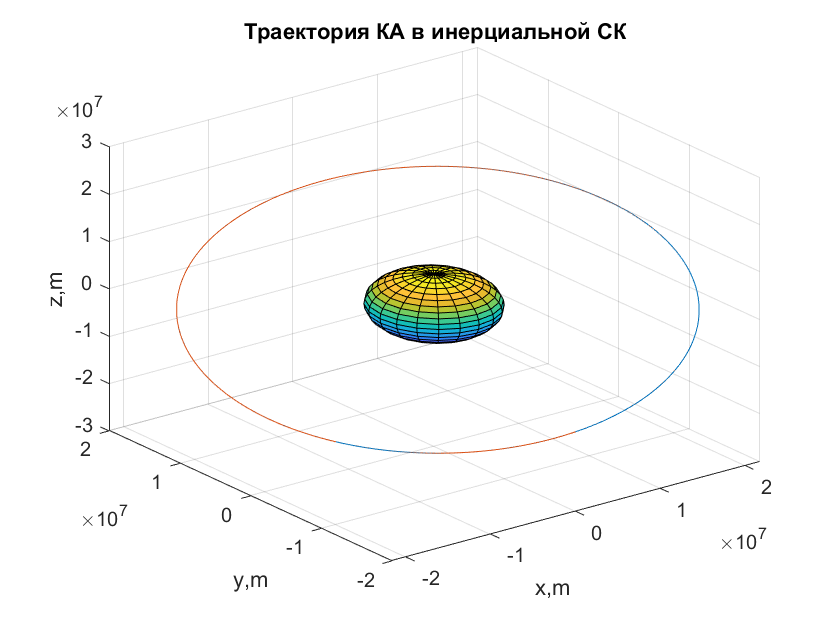
\includegraphics[scale=0.2]{inertz}}
	\caption{Траектория движения в инерциальной СК  }
	\label{inertz}
\end{figure}

\begin{figure}[h!]
	
	\centering{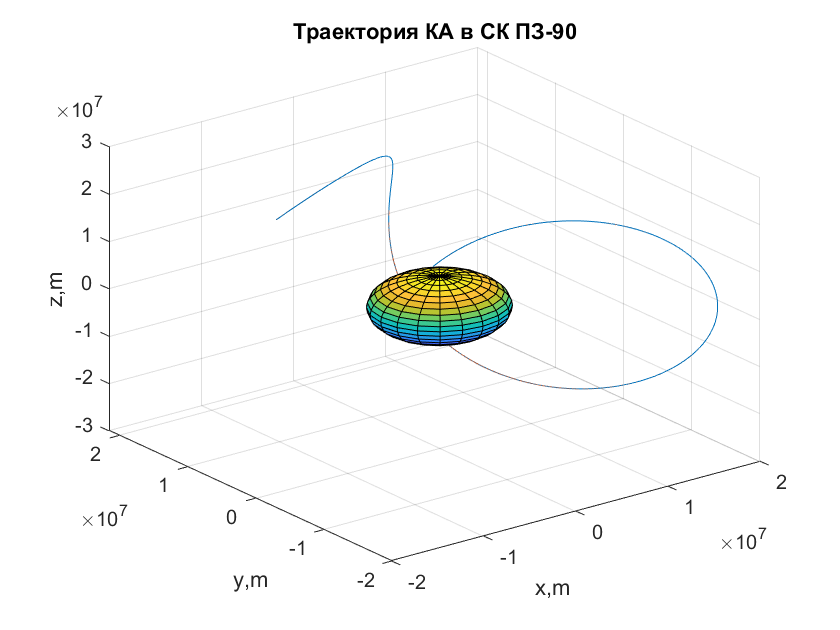
\includegraphics[scale=0.2]{PZ90}}
	\caption{Траектория движения  СК ПЗ-90 }
	\label{PZ}
\end{figure}




\section{Выводы}

На третьем этапе курсового проекта был разработан модуль на языке C++, позволяющий получить координаты НКА на заданный интервал времени для двух СК.  По результатам работы на этапе была получена следующая научно-техничекая продукция:

-программный модуль расчета положения НКА;

-графики траекторий НКА на заданный интервал времени.


\newpage
\addcontentsline{toc}{section}{\bibname}
\begin{thebibliography} {7}
	
	\bibitem{ICD} ИКД Глонасс 5.1, 2008
	\bibitem{alex} Эллайн Алекс, C++. От ламера до программера, 2015.
	

\end{thebibliography}

\end{document}
